\section{Siti di misura e lunghezze d'onda impiegate}
La pelle rappresenta il limite di interazione tra il corpo umano e l'ambiente esterno. Uno dei fattori ambientali con cui interagisce è la luce. L'analisi dell'interazione luce-pelle presenta alcune criticità, a causa dei complessi fenomeni di diffusione, assorbimento e riflessione  delle onde luminose. Di questi, l'assorbimento e la diffusione contribuiscono in modo significativo all'aspetto della pelle. Si stima che circa una percentuale dal 4\% al 7\% della luce visibile sia riflessa dalla superficie epidermica, indipendentemente dalla lunghezza d'onda e dal colore della pelle. La restante parte viene rifratta e assorbita dalla pelle. 
\pagebreak
\subsection{Assorbimento dell'energia luminosa e lunghezze d'onda}
Il fenomeno dell'assorbimento rappresenta una riduzione dell'energia luminosa. Nei tessuti umani questo è dovuto principalmente a due sostanze \cite{Lister2012}.
\begin{itemize}
\item l'emoglobina, spesso indicata con la sigla Hb, è una proteina contenente ferro in grado di combinarsi in modo reversibile con l’ossigeno molecolare \cite{SilverthornDeeUnglaub2020Fu:u}. Come mostrato dalla figura \Fig~\ref{fig:AssorbimentoEmolglobina}, l'emoglobina presenta tre picchi di assorbimento nella regione della luce visibile. Il primo (noto anche come \textit{Picco di Soret}) si trova all'interno della regione blu dello spettro ed è dominante. Gli altri due invece si possono distinguere nella regione giallo-verde, con una lunghezza d'onda compresa tra i 500 e 600 nm. Questi tre picchi combinati danno all'emoglobina un colore rosso;
\item la melanina, contenuta sotto forma di granuli nelle cellule dello strato basale dell’epidermide \cite{SilverthornDeeUnglaub2020Fu:u}. La melanina assorbe principalmente le lunghezze d'onda più corte (\Fig~\ref{fig:PicchiAssorbimento}), quindi presenta uno spettro di assorbimento che decresce gradualmente dall'ultravioletto fino all'infrarosso. In realtà, la melanina è una molecola molto complessa e la sua struttura non è ancora ben nota.
\end{itemize}
\begin{figure}[tb]
	\centering
	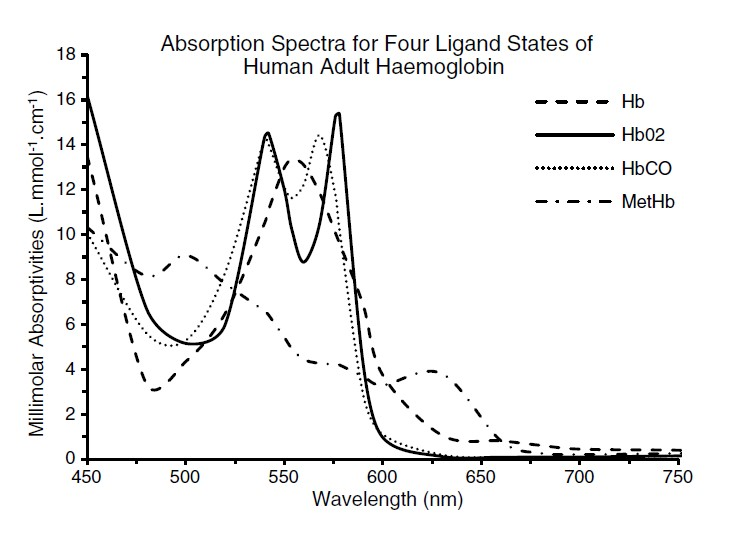
\includegraphics[width=0.8\linewidth]{ImageFiles/Fotopletismografia/AssorbimentoEmolglobina}
	\caption{Spettri di assorbimento di deossiemoglobina (Hb), ossiemoglobina (HbO2), carbossiemoglobina (HbCO), metaemoglobina (MetHb) e emoglobina (Hb) nella regione di luce visibile (immagine tratta da Lister et al.\cite{Lister2012}).}
	\label{fig:AssorbimentoEmolglobina}
\end{figure}
Un altro elemento di cui tener conto è l'acqua che presenta un basso assorbimento nella regione visibile, mentre assorbe la luce nel regime ultravioletto e del lontano infrarosso. 
\begin{figure}[tb]
	\centering
	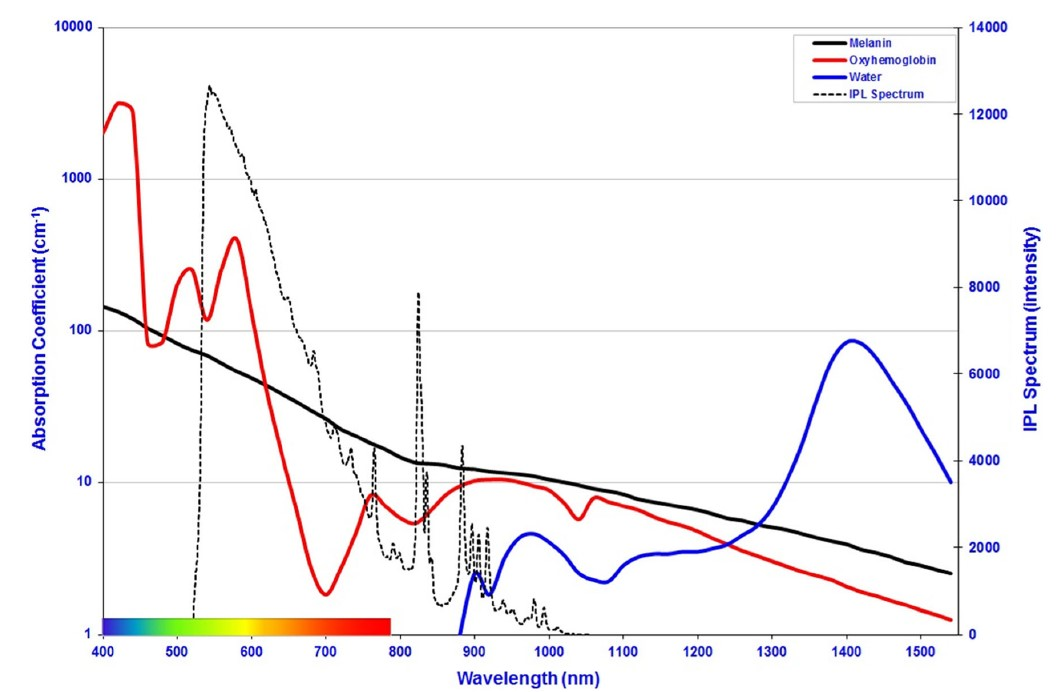
\includegraphics[width=1\linewidth]{ImageFiles/Fotopletismografia/PicchiAssorbimento}
	\caption{Coefficienti di assorbimento dell'ossiemoglobina, melanina, acqua in funzione delle lunghezze d'onda (immagine tratta da Ash et al.\cite{Ash2017}).}
	\label{fig:PicchiAssorbimento}
\end{figure}
Le regioni di luce che riescono ad attraversare maggiormente i tessuti umani sono quindi quella rossa e del vicino infrarosso (\Fig~\ref{fig:PenetrazioneLuce}). Per questo motivo sono spesso utilizzate per applicazioni fotopletismografiche.
\begin{figure}[tb]
	\centering
	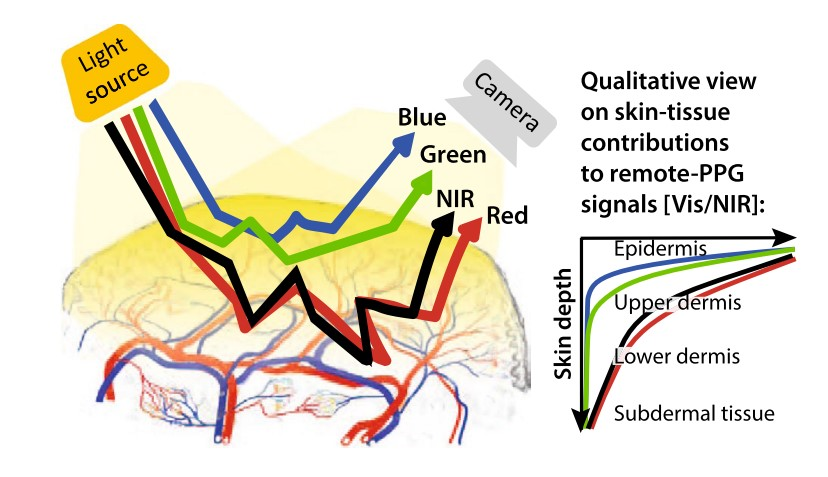
\includegraphics[width=0.8\linewidth]{ImageFiles/Fotopletismografia/PenetrazioneLuce}
	\caption{Profondità nel tessuto raggiunta dalla luce in funzione della lunghezza d'onda (immagine tratta da Moço et al.\cite{Moco2021}).}
	\label{fig:PenetrazioneLuce}
\end{figure}
La profondità nel tessuto umano che si può raggiungere dipende dalla lunghezza d'onda ma anche dalla distanza tra la sorgente luminosa e il foto-rilevatore. Come evidenziato prima, le luce rossa e infrarossa permettono acquisizioni a maggiore profondità nel tessuto. Al contrario la luce verde viene assorbita in quantità superiore\cite{Lee2021} a causa dell'emoglobina e della deossiemoglobina (\Fig~\ref{fig:AssorbimentoEmolglobina}). Infatti, nelle zone in cui il sangue pulsa attraverso la pelle si rileva una variazione tra luce emessa e riflessa maggiore per la regione verde rispetto a quella infrarossa. Questa caratteristica permette di avere un rapporto segnale-rumore (Signal to Noise Ratio), superiore a quello ottenuto con luce infrarossa. Pertanto, la luce verde risulta più adatta per misure superficiali come la variazione del flusso sanguigno superficiale \cite{Youssef2020}.

\clearpage

\subsection{Siti di misura}
La scelta del sito di misura risulta ancora oggi oggetto di discussione dal momento che è difficile definire una zona del corpo migliore per acquisizioni fotopletismografiche. In realtà, la scelta va fatta in base alla tipologia di applicazione e alla qualità dell'acquisizione che si reputa accettabile.
\begin{figure}[b]
	\centering
	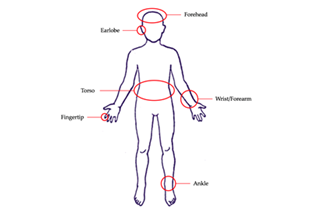
\includegraphics[width=0.6\linewidth]{ImageFiles/Fotopletismografia/ZoneAcquisizione}
	\caption{I principali siti di misura impiegati per segnali PPG (immagine tratta da Ghamari e Mohammad\cite{Ghamari2018}).}
	\label{fig:ZoneAcquisizione}
\end{figure}
Tuttavia ci sono alcune zone che vengono privilegiate per il posizionamento dei sensori PPG.

\textbf{Polpastrello} Rappresenta la zona più comune per acquisizioni e costituiscono un'area ricca di capillari e con una bassa concentrazione di melanina. Per questo motivo è particolarmente adatta a misure in profondità con luce rossa e infrarossa, che permettono misure della frequenza cardiaca e di saturazione di emoglobina.

\textbf{Polso}  Il primo tipo di acquisizioni sul polso utilizza la parte superiore (postero-esterno). In questo punto si ha maggiore presenza di capillari sanguigni. Per queste misure si utilizza principalmente la luce verde dal momento che l'acquisizione da effettuare è di tipo superficiale.	 Il secondo tipo di acquisizione invece è quello che coinvolge la parte inferiore (antero-interna), dove si ha il passaggio delle arterie ulnare e radiale. Questa tipologia di acquisizione permette di ottenere un segnale di buona qualità con tutte e tre le sorgenti luminose. Tuttavia, nei dispositivi commerciali, prevale l'acquisizione sulla faccia postero-esterna poiché sono più agevoli da indossare. Un limite di queste misure è la presenza di disturbi legati al movimento del braccio che però possono essere ridotti tramite l'integrazione di una piattaforma inerziale nel sensore PPG\cite{Ghamari2018}.

\textbf{Fronte} Si tratta di una regione ricca di arterie che si diramano dalla carotide interna \cite{Abay2019}. Per cui le misure in questa zona offrono quindi una buona qualità e affidabilità del segnale. Le acquisizioni sulla fronte sono anche meno sensibili ai disturbi legati al movimento ed è una posizione più accessibile rispetto ai polpastrelli. Questo sito viene utilizzato tipicamente per la misura della saturazione arteriosa di ossigeno.

\textbf{Orecchio} I lobi delle orecchie rappresentano una zona con basso contenuto di cartilagine ed elevata affluenza di sangue. Queste caratteristiche permettono di ottenere dei segnali di buona qualità. Anche per i lobi delle orecchie si ha meno vulnerabilità agli artefatti dovuti al movimento e offrono una posizione comoda. Infatti, i dispositivi di questo tipo sono altamente indossabili\cite{Ghamari2018}. Il sensore PPG può essere posizionato anche all'interno di cuffie e auricolari, che garantiscono un elevato comfort in caso di monitoraggi a lunga durata.

 